\pagestyle{empty}
\chapter*{\centering \large DAFTAR RIWAYAT HIDUP}
\thispagestyle{empty}

\begin{wrapfigure}{l}{4cm}
	\vspace{-25pt}
	\begin{center}
		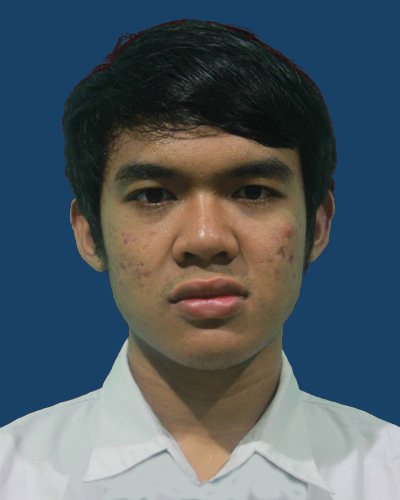
\includegraphics[width=0.27\textwidth]{gambar/pas-foto}
	\end{center}
	\vspace{-80pt}
\end{wrapfigure}

\noindent \textbf{AMELIA APRILIANI.}  Lahir di Jakarta, 23 April 1996.  Anak pertama dari pasangan Bapak H. Nurdin dan Ibu Nurjanah. Saat ini beralamatkan di Jl. Olah Raga I RT.010 RW.05 No.64, Cililitan Jakarta Timur.

\vspace{0.5cm}
\noindent
\begin{center}
	\begin{flushright}
		\begin{tabular}{lcl}
			No. Ponsel	& :&  085776210885 \\
			Email	& :&  ameliaapriliani85@gmail.com
		\end{tabular}
	\end{flushright}
\end{center}
\vspace{0.5cm}

\noindent \textbf{Riwayat Pendidikan} : Penulis mengawali pendidikan di TK As-Saadah pada tahun 2001 - 2002, dan kemudian melanjutkan pendidikan di SDN Cililitan 01 Pagi pada tahun 2002 - 2008. Setelah itu, penulis melanjutkan ke SMPN 150 Jakarta hingga tahun 2011. Kemudian melanjutkan ke SMAN 14 Jakarta pada tahun 2011-2014. Di Tahun 2014 penulis melanjutkan ke Universitas Negeri Jakarta (UNJ), Program Studi Ilmu Komputer, melalui jalur PENMABA. Di akhir tahun 2018 (Hari, ... 2018) penulis telah memperoleh gelar Sarjana Komputer (S.Kom), Program Studi Ilmu Komputer, Fakultas Matematika dan Ilmu Pengetahuan Alam, Universitas Negeri Jakarta.

\noindent \textbf{Riwayat Organisasi} : Selama di bangku perkuliahan, penulis aktif di organisasi keilmiahan Program Studi Ilmu Komputer sebagai anggota merangkap Sekertaris periode 2015-2016. Penulis juga berpartisipasi dalam kegiatan BINER (Be Innovative and Educated Researcher) yaitu kegiatan workshop dan seminar yang diadakan oleh DEFAULT, dimana penulis tergabung sebagai anggota merangkap Sekertaris. 